\section{Supplementary results and figures}

\begin{figure}[tbp]
\centering
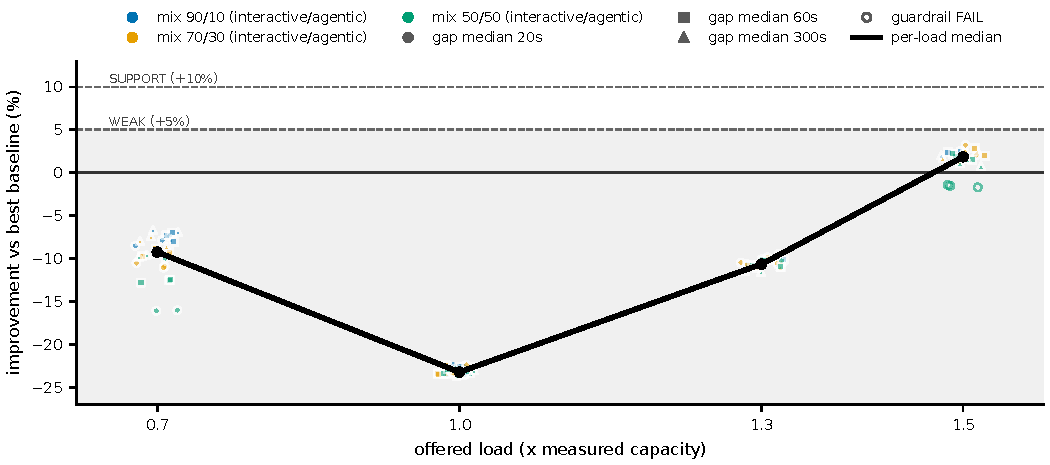
\includegraphics[width=3.25in]{figures/F1_improvement_vs_load.pdf}
\caption{Per-cell improvement of the reservation discipline over the best per-cell tuned baseline, across offered load. Each point is one of 108 pre-registered core cells; the heavy line traces the per-load median. The deficit is U-shaped, deepest at nominal provisioning (22.4 to 23.6 percent at 1.0x), and the sign flips past saturation (+0.8 to +3.2 percent at 1.5x). Dashed lines mark the pre-registered WEAK (+5 percent) and SUPPORT (+10 percent) thresholds; no cell reaches SUPPORT. Open symbols mark the four cells failing the interactive guardrail (Section 6.4).}
\label{fig:improvement}
\end{figure}
\begin{figure}[tbp]
\centering
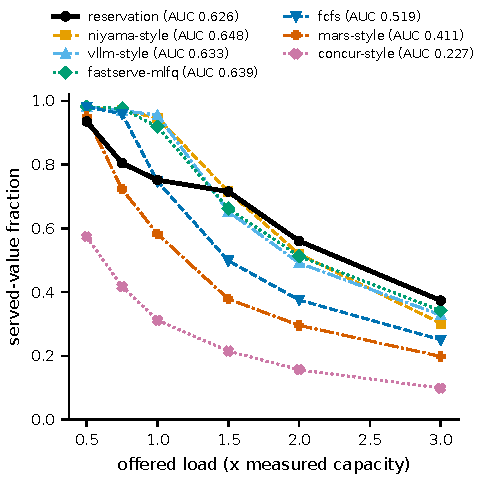
\includegraphics[width=3.25in]{figures/F3_served_value.pdf}
\caption{Served value across the load sweep. The reservation discipline's area under curve (0.626) trails deadline-ordered class scheduling (0.648), killing the graceful-degradation hypothesis; the admission-throttling baselines collapse under overload (Section 6.5).}
\label{fig:servedvalue}
\end{figure}
\begin{figure*}[tbp]
\centering
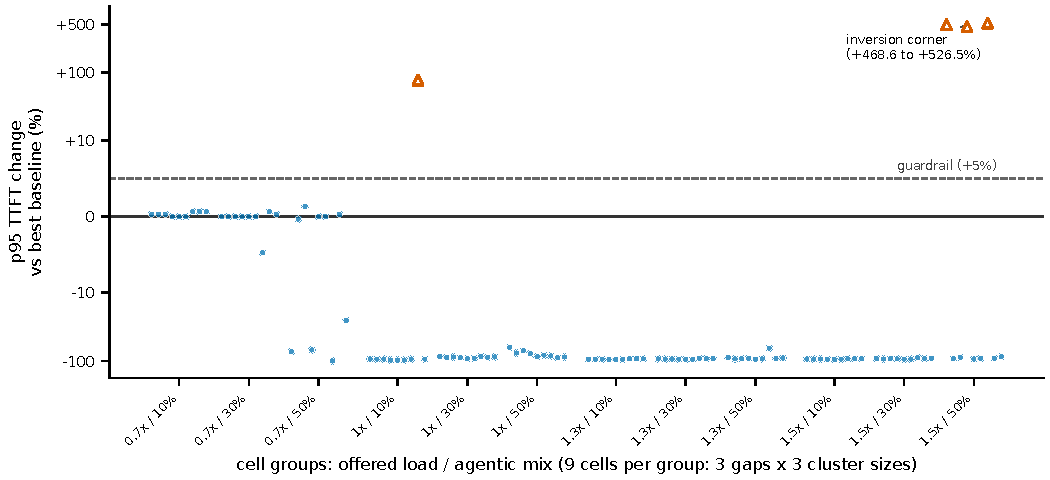
\includegraphics[width=\textwidth]{figures/F2a_interactive_ttft.pdf}
\caption{Interactive tail latency under reservations. Per-cell p95 time-to-first-token change versus the best baseline: at and above nominal load, reservations improve interactive tail latency by 63.3 to 97.1 percent by keeping agentic flows off the shared pool. The effect inverts in the heavy-agentic, overloaded, short-gap corner, where the guardrail fails by 468.6 to 526.5 percent (Section 6.4).}
\label{fig:ttft}
\end{figure*}
\begin{figure}[tbp]
\centering
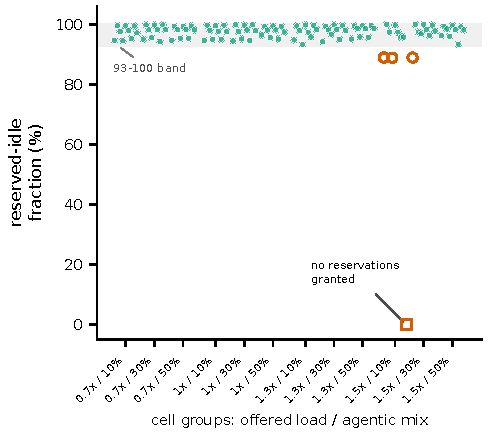
\includegraphics[width=3.25in]{figures/F2b_reserved_idle.pdf}
\caption{What that isolation costs. Reserved-idle fraction per cell: the protection of Figure~\ref{fig:ttft} is priced in capacity held idle, 93 to 100 percent of the reserved pool in 77 of 81 cells, with three load-1.5 cells at 88.9 percent and one cell granted no reservations (marked). This is the structural duty-cycle cost of Section 6.5.}
\label{fig:isolation}
\end{figure}
\begin{table*}[tbp]
\centering
\small
\caption{Policy roster and tuned parameters per workload family (corrected-horizon tuning campaign; 8-point equal-budget grids).}
\label{tab:roster}
\begin{tabular}{llp{4.3in}}
\toprule
policy & workload family & tuned parameters \\
\midrule
concur\_style & mix\_10 & \texttt{additive\_increase=1.0, congestion\_queue\_threshold=0.25, multiplicative\_decrease=0.5} \\
concur\_style & mix\_30 & \texttt{additive\_increase=1.0, congestion\_queue\_threshold=0.25, multiplicative\_decrease=0.5} \\
concur\_style & mix\_50 & \texttt{additive\_increase=1.0, congestion\_queue\_threshold=0.25, multiplicative\_decrease=0.5} \\
fastserve\_mlfq & mix\_10 & \texttt{num\_levels=4, preempt\_mode=swap, quantum\_scale=2.0} \\
fastserve\_mlfq & mix\_30 & \texttt{num\_levels=4, preempt\_mode=swap, quantum\_scale=2.0} \\
fastserve\_mlfq & mix\_50 & \texttt{num\_levels=4, preempt\_mode=swap, quantum\_scale=2.0} \\
fcfs & mix\_10 & \texttt{(no parameters)} \\
fcfs & mix\_30 & \texttt{(no parameters)} \\
fcfs & mix\_50 & \texttt{(no parameters)} \\
mars\_style & mix\_10 & \texttt{additive\_increase=2.0, multiplicative\_decrease=0.75, retain\_threshold\_tokens=500} \\
mars\_style & mix\_30 & \texttt{additive\_increase=2.0, multiplicative\_decrease=0.75, retain\_threshold\_tokens=500} \\
mars\_style & mix\_50 & \texttt{additive\_increase=2.0, multiplicative\_decrease=0.5, retain\_threshold\_tokens=500} \\
niyama\_style & mix\_10 & \texttt{demote\_after\_fraction=1.0, preempt\_mode=swap} \\
niyama\_style & mix\_30 & \texttt{demote\_after\_fraction=1.0, preempt\_mode=swap} \\
niyama\_style & mix\_50 & \texttt{demote\_after\_fraction=1.0, preempt\_mode=swap} \\
reservation & mix\_10 & \texttt{degradation.action=shorten, pin\_mode=tiered, reserved\_subset\_fraction=0.05} \\
reservation & mix\_30 & \texttt{degradation.action=shorten, pin\_mode=tiered, reserved\_subset\_fraction=0.05} \\
reservation & mix\_50 & \texttt{degradation.action=shorten, pin\_mode=strict, reserved\_subset\_fraction=0.05} \\
vllm\_style & mix\_10 & \texttt{max\_batch\_fraction=1.0, preempt\_mode=swap} \\
vllm\_style & mix\_30 & \texttt{max\_batch\_fraction=1.0, preempt\_mode=swap} \\
vllm\_style & mix\_50 & \texttt{max\_batch\_fraction=1.0, preempt\_mode=swap} \\
\bottomrule
\end{tabular}

\end{table*}
\begin{table*}[tbp]
\centering
\small
\caption{Pre-registered verdict summary (thresholds fixed 2026-07-06).}
\label{tab:verdict}
\begin{tabular}{llll}
\toprule
threshold & required & measured & outcome \\
\midrule
median improvement & $\geq$ +10\% (support) / $\geq$ +5\% (weak) & -10.3\% & KILL \\
supporting cells & $\geq$ 60\% of core cells & 0 of 108 (0\%) & KILL \\
interactive guardrail & p95 TTFT degradation $\leq$ 5\% & intact in 96\% of cells & holds (4 cells fail) \\
\bottomrule
\end{tabular}

\end{table*}
\begin{table*}[tbp]
\centering
\footnotesize
\caption{H3 absolute compliant-flow completion rates at each runaway-injection level, with the worst delta versus the no-injection condition (percentage points).}
\label{tab:h3}
\begin{tabular}{lrrrrr}
\toprule
policy & inj 0\% & inj 1\% & inj 5\% & inj 10\% & worst delta \\
\midrule
reservation & 0.503 & 0.475 & 0.499 & 0.471 & -3.1 \\
fcfs & 0.332 & 0.295 & 0.306 & 0.282 & -5.0 \\
mars\_style & 0.249 & 0.223 & 0.245 & 0.227 & -2.6 \\
fastserve\_mlfq & 0.102 & 0.100 & 0.114 & 0.116 & -0.3 \\
concur\_style & 0.082 & 0.082 & 0.070 & 0.063 & -1.9 \\
vllm\_style & 0.000 & 0.000 & 0.000 & 0.000 & +0.0 \\
niyama\_style & 0.000 & 0.000 & 0.000 & 0.000 & +0.0 \\
\bottomrule
\end{tabular}

\end{table*}
\begin{table*}[tbp]
\centering
\footnotesize
\caption{Service-model sensitivity: measured effect and binding classification per constant.}
\label{tab:sens}
\begin{tabular}{llll}
\toprule
constant & perturbation & representative-cell delta & binding \\
\midrule
single-stream decode rate & 0.7x / 1.3x & deficit 21.5\% $\to$ 4.4\% / 13.0\% & binding \\
peak decode rate & $\pm$30\% & none (0 of 19{,}342 decode calls bound) & non-binding \\
cache bytes per token & $\pm$30\% & none (peak HBM near 39\% of capacity) & non-binding \\
\bottomrule
\end{tabular}

\end{table*}

\clearpage
